\documentclass{article}

\usepackage{caption}
\usepackage{subcaption}
\usepackage{graphicx}
\usepackage{tikz}
\usepackage{tikzsymbols}
\usetikzlibrary{calc,patterns}
\usepackage{float}
\usepackage{pdflscape}

\def\centerarc[#1](#2)(#3:#4:#5){\draw[#1] ($(#2)+({#5*cos(#3)},{#5*sin(#3)})$) arc (#3:#4:#5);}

\pagestyle{empty}
\begin{document}
	\centering
	\begin{figure}[H]
			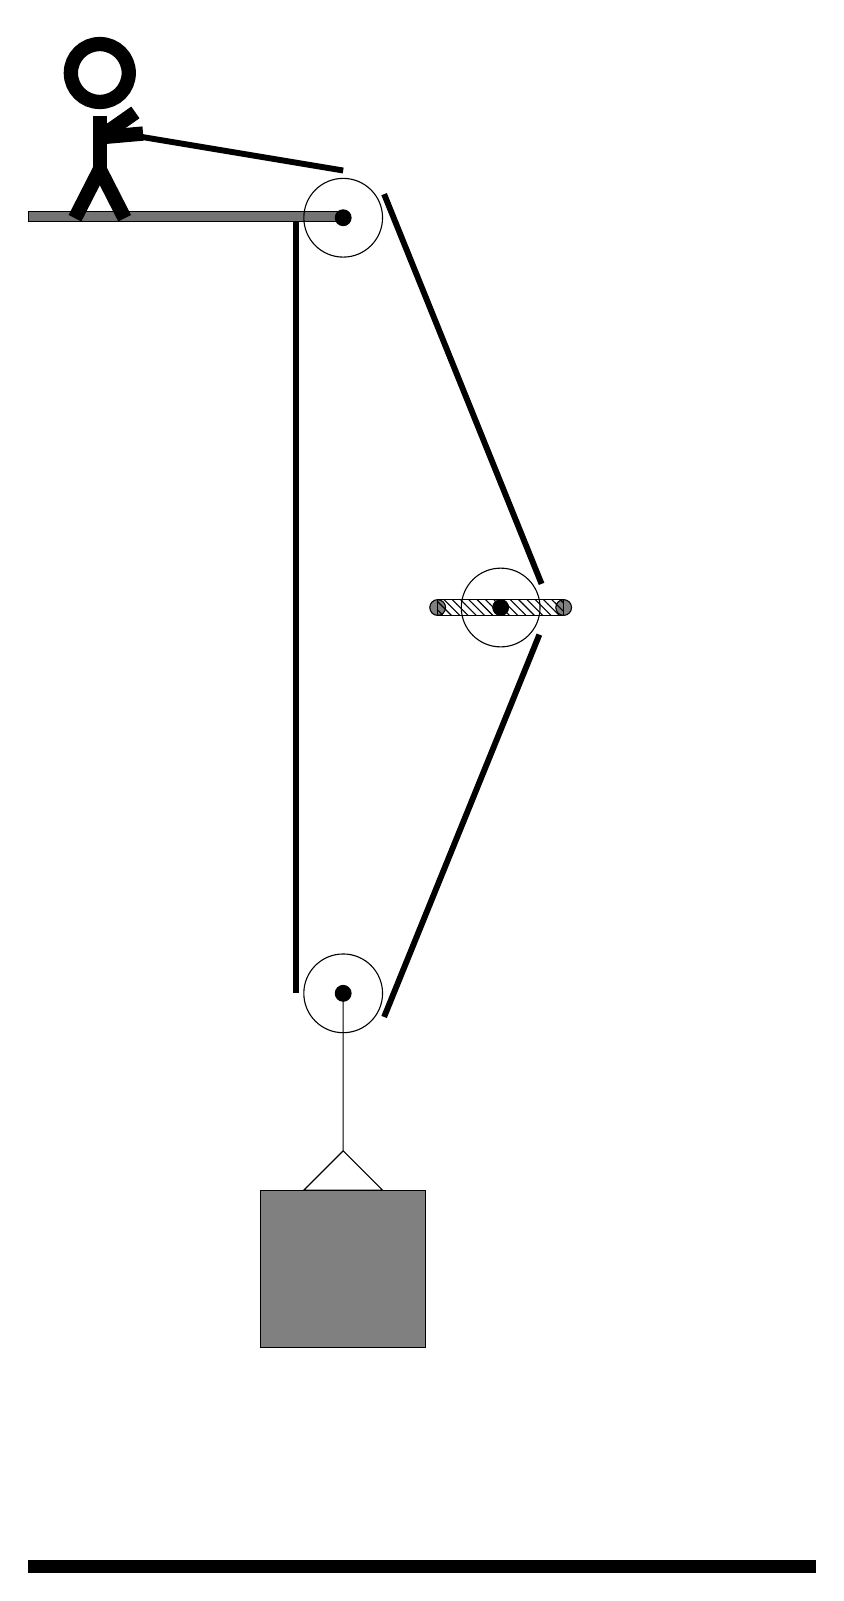
\begin{tikzpicture}
				%%%%% START %%%%%
				\def\a{14}
				\def\radlg{0.5}
				\def\radrp{0.6}
				\def\radsm{0.1}
				\def\yone{\a-\a*0.7}
				\def\xone{2}
				\def\ytwo{\a+0.05}
				\def\xtwo{2}
				\def\xthree{4}
				\def\ythree{\a-\a*0.35}
				\def\dx{-1}
				\def\dy{\a+1.15}
				\def\dw{1.75mm}
				\def\barbump{0.2}
				\def\width{0.75mm}
				
				\draw[fill=black!55] (-2,\a) rectangle (\xtwo,\a+0.125);
				
				\draw (\xone,\yone) circle (\radlg);
				\draw[fill=black] (\xone,\yone) circle (\radsm);
	
				\draw (\xtwo,\ytwo) circle (\radlg);
				\draw[fill=black] (\xtwo,\ytwo) circle (\radsm);
				
				\draw[fill=white](\xthree,\ythree) circle (\radlg);
				\draw[fill=black] (\xthree,\ythree) circle (\radsm);
				\draw[fill=black!50] (\xthree-\radrp-\barbump,\ythree) circle (\radsm);
				\draw[fill=black!50] (\xthree+\radrp+\barbump,\ythree) circle (\radsm);
				\draw[pattern=north west lines, pattern color=black] (\xthree-\radrp-\barbump,\ythree+0.1) rectangle (\xthree+\radrp+\barbump,\ythree-0.1); 
				
				\draw (\xone,\yone) -- (\xone,\yone-2) -- (\xone-0.5,\yone-2.5) -- (\xone+0.5,\yone-2.5) -- (\xone,\yone-2);
				\draw[fill=black!50] (\xone-1.05,\yone-2.5) rectangle (\xone+1.05,\yone-4.5);  
				
				\draw[line width=\width] (\xone-\radrp,\a) -- (\xone-\radrp,\yone); 
				\centerarc[line width=\width](\xone,\yone)(180:330:\radrp);
				\draw[line width=\width]({\xone+\radrp*cos(330)},{\yone+\radrp*sin(330)}) -- ({\xthree+\radrp*cos(325)},{\ythree+\radrp*sin(325)});
				\centerarc[line width=\width](\xthree,\ythree)(390:325:\radrp);
				\draw[line width=\width]({\xthree+\radrp*cos(390)},{\ythree+\radrp*sin(390)}) -- ({\xtwo+\radrp*cos(390)},{\ytwo+\radrp*sin(390)});
				\centerarc[line width=\width](\xtwo,\ytwo)(30:90:\radrp);
				\draw[line width=\width](\xtwo,\ytwo+\radrp) -- (\dx,\dy);
					
				\node at (\dx,\dy) {\Strichmaxerl[10][-175][35]};
				
				\draw[fill=black] (-2,-3) rectangle (8,-3.15);
				%%%%% END %%%%%
			\end{tikzpicture}
	\end{figure}
	
\end{document}